\documentclass[lettersize,journal]{IEEEtran}
\usepackage{amsmath,amsfonts}
\usepackage{algorithmic}
\usepackage{algorithm}
\usepackage{array}
\usepackage[caption=false,font=normalsize,labelfont=sf,textfont=sf]{subfig}
\usepackage{textcomp}
\usepackage{stfloats}
\usepackage{url}
\usepackage{verbatim}
\usepackage{graphicx}
\usepackage{cite}

% added packages from authors
\usepackage{xcolor}
\usepackage{booktabs} % for \midrule in tables
\usepackage{hhline}
\usepackage{bbm}
\usepackage{bm}
\usepackage{makecell}
\usepackage[mode=buildnew]{standalone}
\usepackage{tikz}
\usetikzlibrary{calc,arrows,patterns,intersections}
\newcommand{\red}[1]{\textcolor{red}{#1}}
\usepackage{pgfplots}
\usepackage{xcolor}
\usepgfplotslibrary{fillbetween}

\hyphenation{op-tical net-works semi-conduc-tor IEEE-Xplore}

\begin{document}


\title{Synergy Among Flexible Demands: Form a Coalition to Earn More from Reserve Market}

\author{Peter A.V. Gade\textsuperscript{*}\textsuperscript{\textdagger}, Trygve Skjøtskift\textsuperscript{\textdagger}, Henrik W. Bindner\textsuperscript{*}, Jalal Kazempour\textsuperscript{*} \\
    \textsuperscript{*}Department of Wind and Energy Systems, Technical University of Denmark, Kgs. Lyngby, Denmark \\
    \textsuperscript{\textdagger}IBM Client Innovation Center, Copenhagen, Denmark
    % <-this % stops a space
    \thanks{
        %Corresponding author. Tel.: +45 24263865. \\ 
        Email addresses: pega@dtu.dk (P.A.V. Gade), Trygve.Skjotskift@ibm.com (T. Skjøtskift), hwbi@dtu.dk (H.W. Bindner), jalal@dtu.dk (J. Kazempour).}% <-this % stops a space
    %    \thanks{Manuscript received April 19, 2021; revised August 16, 2021.} \\

    \vspace{-8mm}
}

% \footnote{Corresponding author. Tel.: +45 24263865. \\ Email addresses: pega@dtu.dk (P.A.V. Gade), Trygve.Skjotskift@ibm.com (T. Skjøtskift), hwbi@dtu.dk (H.W. Bindner), jalal@dtu.dk (J. Kazempour).}

% The paper headers
%\markboth{Journal of \LaTeX\ Class Files,~Vol.~14, No.~8, August~2021}%{Shell \MakeLowercase{\textit{et al.}}: A Sample Article Using IEEEtran.cls for IEEE Journals}

%\IEEEpubid{0000--0000/00\$00.00~\copyright~2021 IEEE}
% Remember, if you use this you must call \IEEEpubidadjcol in the second
% column for its text to clear the IEEEpubid mark.

\maketitle

% \tableofcontents

\begin{abstract}
    % It has been well shown how demand-side flexibility can provide services to the power grid through an aggregator with no emissions. However, the aggregator still faces two, mostly unexplored, fundamental problems: 1) how many demand-side assets are needed in order to achieve a synergy effect? And 2) how are payments allocated to individual flexible demands downstream of the aggregator? This paper answers these two questions using simulations of uncertain assets to illustrate the synergy effect, and Shapley values are used as a payment allocation mechanism. As a use case, manual frequency restoration reserves (mFRR) are used as the ancillary service targeted by the aggregator with real prices from 2022.
    We show how flexible demands can earn more collectively than individually by forming a coalition and bidding to the reserve market. This synergy effect is quantified as a function of the number of homogeneous assets in the coalition. Flexible demands, together as a single participant, bid to the manual Frequency Restoration Reserve (mFRR) market. A subsequent payment allocation mechanism using Shapley values is proposed to distribute the earning among demands, while incentivizing them to remain in the coalition. For our numerical study, we use real price data from the Danish mFRR market. The value of synergy is explored by varying the penalty for missed delivery of flexibility.
\end{abstract}

\begin{IEEEkeywords}
    Demand-side flexibility, Synergy effect, manual frequency restoration reserve, Shapley values, payment allocation
\end{IEEEkeywords}

% TO BE DELETED
\tableofcontents

\section{Introduction}\label{sec:Introduction}

It has been extensively addressed in the literature how flexible demands can provide ancillary services to the power grid through an aggregator \cite{biegel2014value}, \cite{macdonald2020demand}, \cite{balijepalli2011review}.
The key is that these services must explicitly be provided using baseline forecasts for the aggregator's flexibility for stochastic flexible resources, including demand-side flexibility, as prescribed in the official documentation for pre-qualification to ancillary services by  the Danish Transmission System Operator (TSO), Energinet \cite{energinet:prequalification}. Thus, aggregation of flexible assets is incentivized not only due to meeting minimum bid requirements \cite{energinet:Systemydelser} but also due to the potential synergy effect of the aggregation.

Several private initiatives for providing demand-side flexibility take place already in Denmark. For example, IBM is spearheading these with their Flex Platform which connects, controls, and aggregates heterogenous assets in the commercial and industrial sector. This aggregated flexibility is monetized through ancillary services such as mFRR (see Section \ref{sec:mFRR}). The flexible consumers providing this flexibility, also called \textit{flexible demands}, earn money from this and can potentially include $CO_{2}$ savings in their accounting.

Aggregation platforms such as the Flex Platform face two fundamental problems: 1) How many demand-side assets are needed in order to achieve a synergy effect by providing a reliable flexibility estimation as prescribed by the TSO? And 2) How are payments allocated to individual flexible demands within the aggregator portfolio downstream of the aggregator?

The first question is answered using a stylized example of uncertain demand by quantifying the synergy effect versus the number of assets required in an aggregator portfolio. We show how individual assets are inherently unpredictable on their own but predictable within a portfolio.

The second question is answered by proposing Shapley values \cite{shapley1997value} as a mechanism to pay flexible demands for their contribution to the portfolio. This provides economic properties such as individual rationality and budget balance that incentivize flexible demands to stay in the aggregator portfolio, i.e., \textit{coalition}, as opposed to act selfishly. This payment is illustrated through an example of six flexible demands, each with numerous assets, in a coalition which an aggregator use for mFRR bidding. In this example, the first flexible provider only provides flexible capacity but no actual up-regulation. In this way, the penalty for doing so can be varied to assess the contribution of the flexible provider to the coalition.

\IEEEpubidadjcol

\subsection{Research questions}

Thus, we aim to answer the following research questions:

\begin{itemize}
    \item How can the synergy effect be quantified for a portfolio of uncertain demand-side assets used for mFRR bidding?
    \item How can payments be fairly allocated to flexible demands in an aggregator portfolio used for mFRR bidding such that each flexible provider is incentived to remain in the portfolio?
\end{itemize}

Simulations are used to answer these questions but with real price data for mFRR in Denmark from 2022.

\subsection{Literature review}

While many have studied important aspects of demand-side flexibility such as feasibility and controllability \cite{bondy2018redefining}, \cite{bondy2017performance}, \cite{bondy2016procedure}, \cite{bondy2014performance}, \cite{biegel2014integration}, \cite{AchievingControllabilityofElectricLoads}. However, an important aspect has been largely overlooked in the literature which is the synergy effect related to aggregating a portfolio of demand-side assets (freezers, heat pumps, ventilation systems, etc.).

In \cite{biegel2014value}, the authors investigate the value of flexible consumption but do not touch upon the synergy effect of a portfolio of assets although it is mentioned that market barriers exist such as the minimum size of a portfolio.

In \cite{pedersen2014aggregation}, it shown how a portfolio of supermarkets can deliver a granular power response which is made possible by the number of supermarkets and their assets within. Although not mentioned explicitly, this is indeed also a form of synergy effect because an aggregator requires a certain number of controllable assets to deliver a granular power response. However, the estimation and value of flexibility \textit{ex-ante} is not tied together with any synergy effect.

Moreover, demand-side synergy is known in other domains such as strategic and organizational diversification \cite{ye2012achieving}, but here we specifically address demand-side flexibility for ancillary services.

For flexible demand, estimating baselines are extremely important since demand does not have an operational baseline schedule like a generation unit \cite{gade2022ecosystem}. In this context, there are two baselines that are relevant: 1) the baseline from which the aggregator estimates its flexible capacity, as prescribed by the Danish TSO \cite{energinet:prequalification} and 2) the baseline that estimates the counterfactual consumption when flexible demand delivers its capacity. 

In our work, we show how the first problem becomes much easier due to the synergy effect of adding assets to the portfolio. The second problem has been studied extensively. In \cite{ziras2021baselines}, the authors explain why baselines are not suited for flexibility in the distribution grid whereas \cite{capacity_limitation_services} instead shows how capacity limitation is another mechanism that works better. 

However, for transmission level ancillary services that deal with balancing production and demand at 50 Hz, baselines are generally accepted as a necessary evil (for demand-side flexibility). Others have tried to come up with exotic mechanisms as alternatives. In \cite{muthirayan2019mechanism}, one such mechanism is provided where the aggregator relies on self-reported baselines from its flexible demands (or agents) which removes the incentive to inflate baselines. In our setting, this is not realistic since flexible demands have no capability to report their own baselines in the first place (remember, they all have other primary business purposes). Therefore, the aggregator has no incentive to inflate any of its flexible demands' baselines anyway. 

In our work, we only rely on baseline estimation on the portfolio level. Then Shapley values \cite{shapley1997value} are used as a mechanism to allocate payments to flexible demands within the portfolio as opposed to using baseline forecasts per flexible demand.


\subsection{Our contribution}

As mentioned, we show two results related to the synergy effect of aggregating many individual demand-side assets with uncertain power consumption. The first is purely statistical and related to the estimation of reserve capacity from the aggregated portfolio versus the individual assets. The second result utilizes the synergy effect of individual \textit{coalitions} of flexibility providers within a portfolio to allocate payments using Shapley values. They provide a useful way for an aggregator to assess the performance of flexibility providers within its portfolio and directly allocate payments in an ex-post setting.

\subsection{Paper structure}

The rest of the paper is organized as follows.

First, the simulation setup is introduced. This includes a brief introduction to the mFRR ancillary services, how demand-side assets are simulated, and how Shapley values work as a payment mechanism in this context. Second, results are shown for the synergy effect of number of assets and the payment allocation mechanism. Third, a brief section on future work outlines the key things absent from this paper which can readily be studied further. Lastly, a conclusion is presented.

\section{Simulation setup}

This section explains the simulation setup in detail. First, a short introduction to mFRR in Denmark is given. For more detailed information of mFRR, see \cite{energinet:Systemydelser}, \cite{energinet:prequalification}, and \cite{energinet:tender_conditions_reserves}.

\subsection{mFRR}\label{sec:mFRR}

Ancillary services are used to balance the power grid such that production meets demand to keep the power grid frequency at 50 Hz\footnote{60 Hz in the US.}. In Denmark, mFRR is deployed after fast frequency services when a frequency drop occurs, i.e., mFRR is only used for up-regulation. mFRR participants are paid according to their capacity and their up-regulation. Often, mFRR providers are not required to up-regulate so their capacity payment constitute a passive income. In our setup, we apply a penalty when the capacity does not match actual up-regulation. For a demand-side aggregator, this could be due to improper capacity estimation or unexpected errors when dispatching assets for up-regulation, e.g., violation of temperature thresholds for TCLs. Bid prices are ignore for simplicity.

We use mFRR reserve prices, balancing prices, and spot prices from DK1\footnote{Western Denmark price zone.} \cite{energinet:energidataservice}, denoted by $\lambda_{h}^{\text{mFRR}}$, $\lambda_{h}^{\text{b}}$, and $\lambda_{h}^{\text{s}}$ respectively. The constant penalty price for not delivering promised capacity is denoted $\lambda^{\text{p}}$.

The aggregator objective function for mFRR bidding can be written:

\begin{align}\label{eq:mFRRObjective}
     & - \underbrace{\sum_{h=1}^{24} \lambda^{\text{s}}_{h}P^{\text{Base}}_{h}}_{\textrm{Energy cost}} + \underbrace{\sum_{h=1}^{24}\lambda_{h}^{\text{mFRR}} p^{\text{mFRR}}_{h}}_{\textrm{Reservation payment}}  \notag \\ & \quad \quad + \underbrace{\sum_{h=1}^{24}  \lambda_{h}^{\text{b}} p^{\text{b},\uparrow}_{h}}_{\textrm{Activation payment}} - \underbrace{\sum_{h=1}^{24}  \lambda_{h}^{\text{b}} p^{\text{b},\downarrow}_{h}}_{\textrm{Rebound cost}} - \underbrace{ \sum_{h=1}^{24}  \lambda^{\text{p}}s_{h}}_{\textrm{Penalty cost}}
\end{align}

Here, $p^{\text{mFRR}}_{h}$ is the hourly mFRR capacity of the aggregator portfolio, $p_{h}^{\text{b},\uparrow}$ is the real-time up-regulation, $p_{h}^{\text{b},\downarrow}$ is the rebound, $s_{h}$ is the energy not delivered, and $p^{\text{Base}}$ the normal operational baseline consumption.

To simplify, we ignore the rebound, i.e., $\lambda_{h}^{\text{b}, \downarrow} = 0$ $\forall{h}$. Also, the energy cost is constant and is not affected by mFRR bidding. Thus, only the reserve and activation payments are considered together with the penalty cost. The profit from mFRR bidding is simply then:

\begin{align}\label{eq:mFRR_profit}
     & \underbrace{\sum_{h=1}^{24}\lambda_{h}^{\text{mFRR}} p^{\text{mFRR}}_{h}}_{\textrm{Reservation payment}} + \underbrace{\sum_{h=1}^{24}  \lambda_{h}^{\text{b}} p^{\text{b},\uparrow}_{h}}_{\textrm{Activation payment}} - \underbrace{ \sum_{h=1}^{24}  \lambda^{\text{p}}s_{h}}_{\textrm{Penalty cost}}
\end{align}

The challenge for the aggregator in eq. (\ref{eq:mFRR_profit}) is therefore two-fold: 1) $p^{\text{mFRR}}_{h}$ must be estimated and 2) $s_{h}$ should be minimized.

In reality, there is also a bidding process for both capacity and up-regulation but, as mentioned, it is ignored here for simplicity. Furthermore, as alluded to in Section \ref{sec:Introduction}, we do not consider the control aspect of the portfolio, i.e., the challenge of effectively following the required response within an hour of up-regulation (although there is also a synergy effect there).

\subsection{Demand-side assets}

In eq. (\ref{eq:mFRR_profit}), the power variables show total power for the whole aggregator portfolio. Each asset, $i$, in the portfolio has its own power consumption, $p_{h, i}$ $\forall{i} \in \mathcal{I}$. Hence:

\begin{subequations}
    \begin{align}
        p^{\text{mFRR}}_{h}        & = \sum_{h=1}^{24} p^{\text{mFRR}}_{h, i}        \\
        p^{\text{b}, \uparrow}_{h} & = \sum_{h=1}^{24} p^{\text{b}, \uparrow}_{h, i} \\
        s_{h}                      & = \sum_{h=1}^{24} s_{h, i}
    \end{align}
\end{subequations}

An asset is defined as any power consuming device\footnote{This including batteries in principle, but these are ignored here.} such as a heat pump, freezer, ventilation system, air condition unit, or boiler, etc. The aggregator can also have high-consuming assets such as a zinc galvanizing furnace, a swimming pool, waste-water centrifugation units, etc.

To keep it simple, we consider assets that deviates from their operational baseline consumption in a uniform manner:

\begin{align}\label{eq:uniform}
    p_{h,i} \thinspace [\text{kW}] = \begin{cases}
                                         1 & \text{if} \quad h = h^{\prime} \sim \mathcal{U}(1,24) \\
                                         0 & \text{otherwise}
                                     \end{cases}
\end{align}

An asset in eq. (\ref{eq:uniform}) could for example be a ventilation unit that is turned on randomly for one hour each day. For an aggregator, it is therefore not possible to estimate $p^{\text{mFRR}}_{h, i}$ accurately, but as $|\mathcal{I}|$ increases, the portfolio consumption converges to a predictable uniform consumption for all $h \in \{1 \hdots 24 \}$ so $p^{\text{mFRR}}_{h}$ becomes predictable. Here, predictable simply means predicting tomorrow's power consumption based on today but more advanced methods can be used \cite{ziras2021baselines}.


This is of course a stylized example as most assets have some degree of predictability, but it is sufficient to show a very relevant problem for aggregators of small-scale, uncertain demand-side assets: in the beginning, the aggregator cannot estimate the reserve capacity of the portfolio, but as the number of assets increases, it becomes much easier.

Furthermore, our definition of an asset is valid for any type of asset, including TCLs. For example, freezers might consume an extra, unexpected amount of energy due to food refills or other exogenous events. Also, the temperature thresholds might be violated which renders flexibility provision impossible. This situation is simulated as explained in the next section.

With profit being defined as in eq. (\ref{eq:mFRR_profit}), the synergy effect of the portfolio is then:

\begin{align}\label{eq:synergy_effect}
    \text{Synergy effect [\%]} = \frac{ \text{Portfolio profit} }{ \sum_{i \in \mathbb{I}} \text{Asset \textit{i} profit} }
\end{align}

Hence, the synergy effect is simply the ratio between the portfolio profit and the sum of individual asset profits. The difference between the two will be due to the activation payment and the penalty cost as the reservation payments are the same.

\subsection{Shapley as a payment mechanism}

The Shapley value is a mechanism to allocate contributions in a cooperative game \cite{shapley1997value}. This idea fits perfectly with the concept of synergy effect in a portfolio of demand-side assets. Now, however, we consider a downstream problem of the aggregator, i.e., how much each flexible demand (with their assets) contributes to the whole portfolio \textit{ex-post} mFRR bidding. Hence, the aggregator has received a pot of money for the whole portfolio, i.e., eq. (\ref{eq:mFRR_profit}), and faces the problem of distributing it to the flexible demands.

To formalize this problem, we let $g \in \mathcal{G} = \{1 \hdots M \}$ denote a flexible provider in the set of all flexible demands with cardinality $M$. The set of assets belonging to $g$ are denoted $\mathcal{A}_{g,i} = \{1 \hdots N_g \}$. The assets are simulated using eq. (\ref{eq:uniform}).

Now, the Shapley value for flexible provider $g$ is given by \cite{shapley1997value}:

\begin{align}\label{eq:shap}
    \phi_g & = \frac{1}{M} \sum_{\mathcal{S} \subseteq \mathcal{G}, g \in \mathcal{S}}\left(\begin{array}{c}
                                                                                                    M-1 \\
                                                                                                    |\mathcal{S}|-1
                                                                                                \end{array}\right)^{-1}[v(\mathcal{S})-v(\mathcal{S} \backslash\{i\})]
\end{align}

Here, $v$ is simply the profit in eq. (\ref{eq:mFRR_profit}). Thus, $v(\mathcal{S})$ represents the value of mFRR bidding for the portfolio of flexible demands given by the coalition $\mathcal{S}$. The value of the grand coalition, i.e., the whole portfolio is given by $v(\mathcal{G}) = \sum_{g \in \mathcal{G}} \phi_{g}$.

The Shapley value  in eq. (\ref{eq:shap}) can be thought of as the average marginal contribution of flexible provider $g$ across all possible coalitions in $\mathcal{G}$. It can only be computed exactly for small $M$ as the number of possible coalitions is equal to $2^{M} - 1$. As $M$ grows, Shapley values can be approximated \cite{castro2009polynomial}.

Using Shapley values as payments, the aggregator have a fair method for allocation. If one flexible provider has assets that marginally contribute with only some flexibility, it will be reflected in their Shapley value. For example, a flexible provider can have a relatively small portfolio of assets. More interestingly, a flexible provider can have many high-consuming assets that for some reason are not up-regulating when needed (as illustrated in Section \ref{sec:Results}). Using Shapley values, the aggregator can ex-post determine how much such a flexible provider contributes with. Otherwise, that can be difficult to estimate for the aggregator due to the benefit of reserve payment versus risk of not being able to up-regulate.

Furthermore, the Shapley value has desirable economic properties such as individual rationality (see Section \ref{sec:Results}) and budget balance.

\section{Results}\label{sec:Results}

In this section, we first show the assets being simulated and the flexible demands (groups) within the aggregated portfolio. Then results for the synergy effect is shown when the number of assets in the portfolio increases. Afterwards, we consider the payment allocation to flexible demands and investigate the impact of a flexible provider not delivering any up-regulation but only capacity.

\subsection{Visualization of groups and assets}

Figure \ref{fig:assets} shows the portfolio consumption. It is almost uniform and fairly predictable where each group is less predictable and each asset within each group even more so. The aggregated distribution approaches a uniform distribution as the number of assets increases.

\begin{figure}[!t]
    \centering
    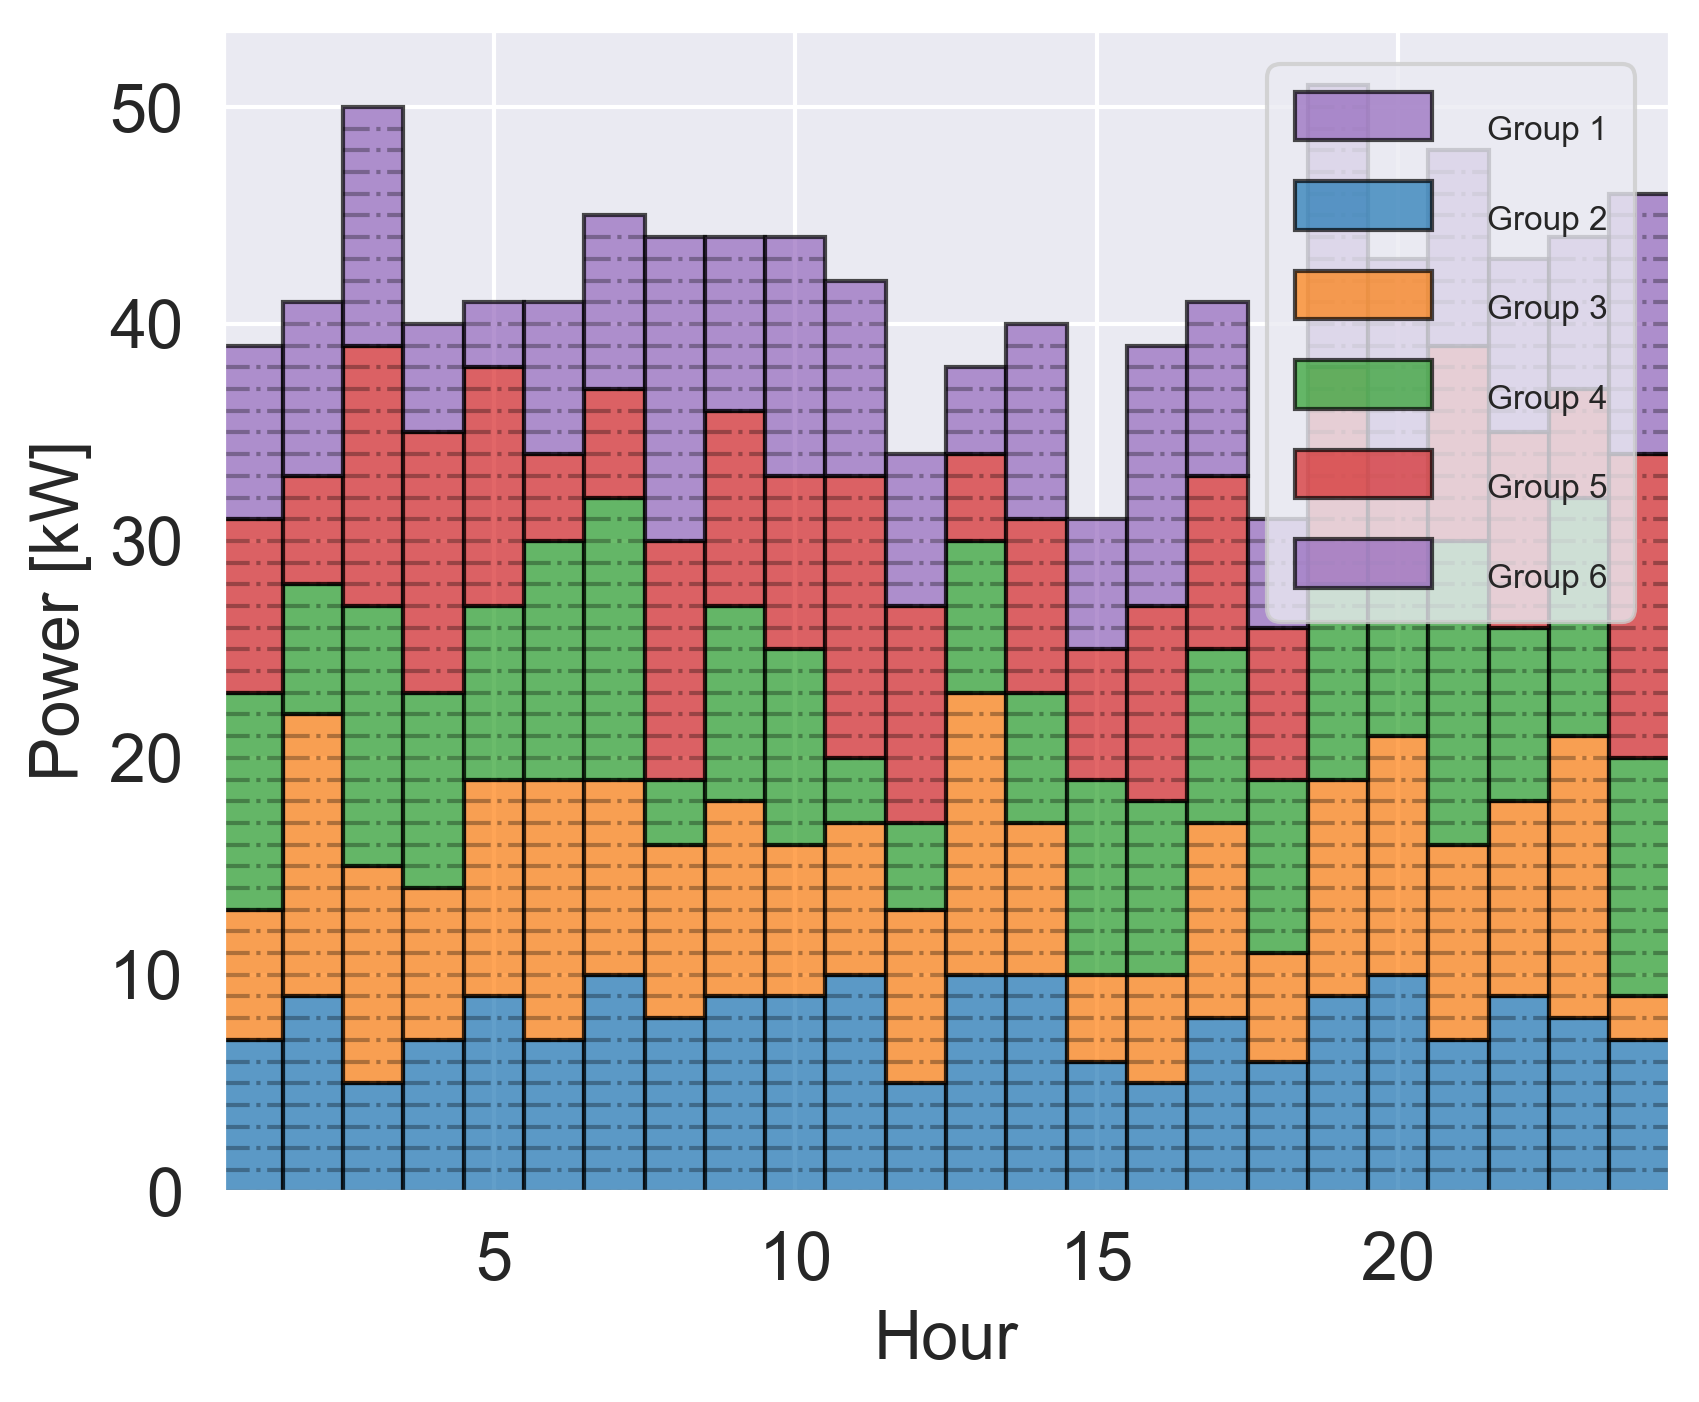
\includegraphics[width=\columnwidth]{figures/assets2.png}
    \caption{Simulation of power consumption of 1000 assets using eq. (\ref{eq:uniform}) with six flexible demands that each has a group of assets (assets are represented as small rectangles within each group).}
    \label{fig:assets}
\end{figure}

\subsection{Synergy effect of assets}

Figure \ref{fig:synergy_effect} shows the simulation of the synergy effect using eq. (\ref{eq:uniform}) and 
eq. (\ref{eq:synergy_effect}) for up to 1000 assets. Even with such uncertain assets, it only takes around 150 of these before the synergy effect flattens. In reality, much fewer assets are then needed to estimate their reserve capacity due to many real-life assets having a more predictable consumption than here..

As discussed already, this of course ignores the synergy effect of controlling assets \textit{within} each hour to deliver a proper response. This probably requires a significant number of assets if all of them are ON/OFF controlled and if they are very heterogenous.

\begin{figure}[!t]
    \centering
    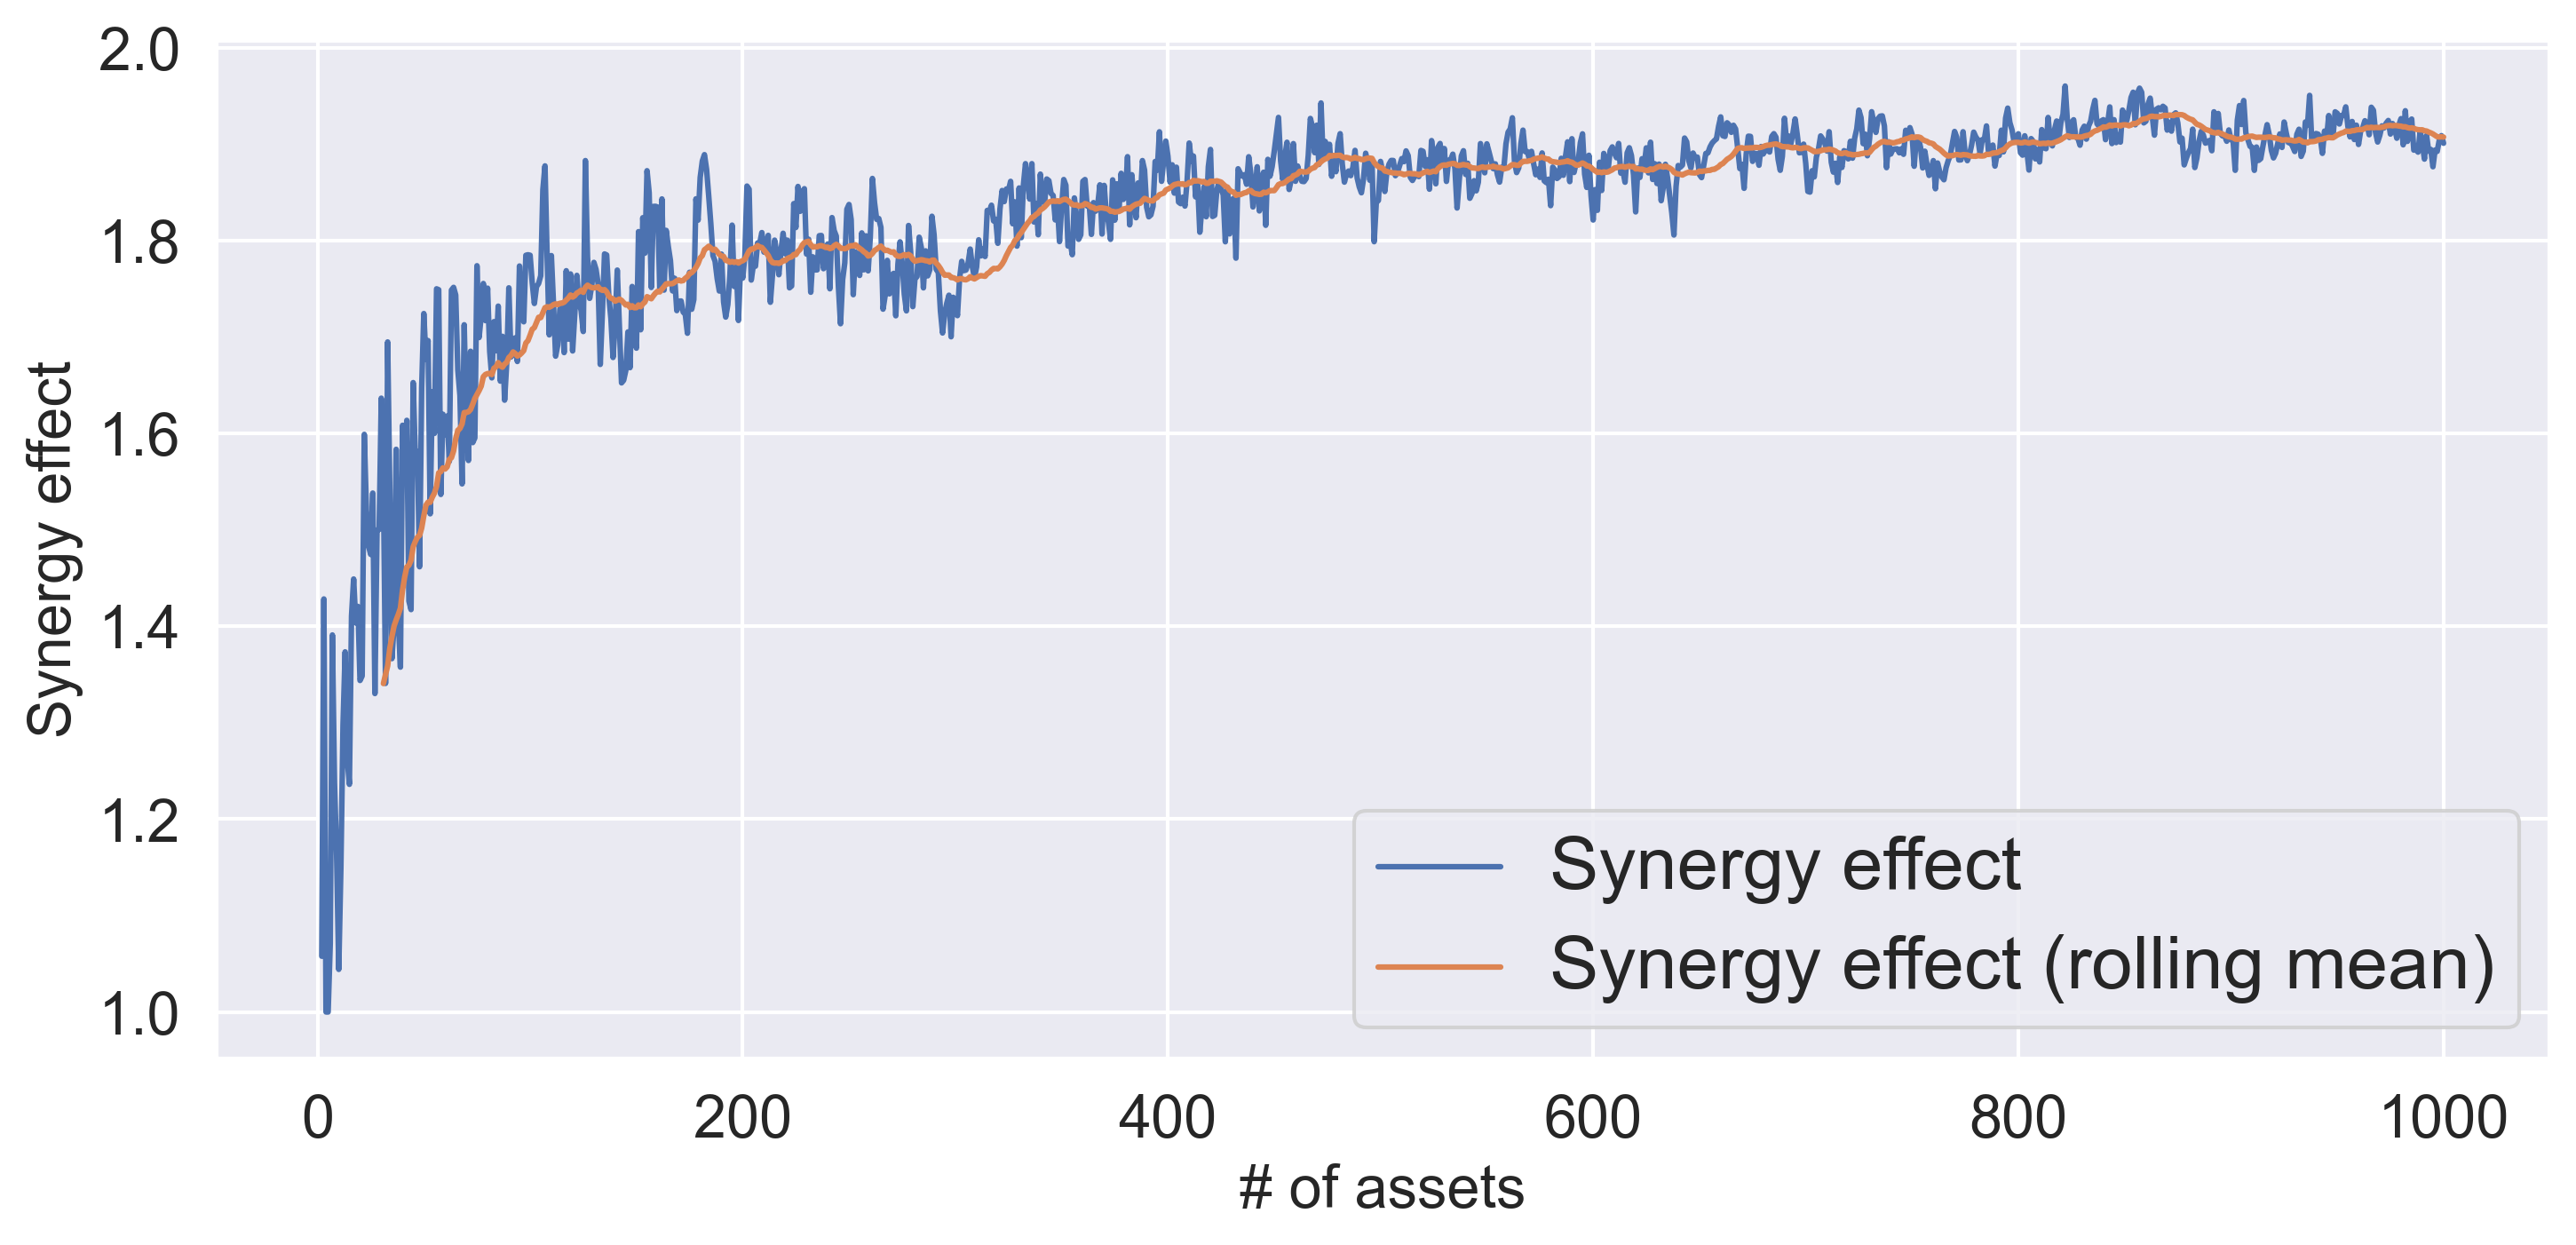
\includegraphics[width=\columnwidth]{figures/synergy_effect.png}
    \caption{Simulation of the impact on the synergy effect by increasing the number of assets. The rolling mean shows the average of the past 40 values.}
    \label{fig:synergy_effect}
\end{figure}

\subsection{Payment allocation}

Figure \ref{fig:shapley_values} shows the Shapley values for a simulation with $M = 6$, and where $g = 1$ has assets that never up-regulates and only contributes with their reserve capacity (which can never be utilized). The simulation is run for increasing values of the penalty parameter, $\lambda^{\text{p}}$.

Interestingly, it shows that $g_1$ actually contribute positively to the portfolio when $\lambda^{\text{p}} < 1.5$. This is simply explained by the price data and how often actual up-regulation is needed (which happens when $\lambda^{\text{b}} > \lambda^{\text{s}}$). If the power grid would need much more up-regulation, the cutoff for $\lambda^{\text{p}}$ would be lower.

The green and orange lines show individual rationality for coalition $G / \{1\}$. The orange line shows the total payment to $G / \{1\}$ when $g_1$ is included in the coalition, and the green line shows the total payment to $G / \{1\}$ when $g_1$ is \textit{not} included in the coalition. Intriguingly, it shows that $G / \{1\}$ benefits from having $g_1$ in the coalition even though $g_1$ gets negative payments. Hence, $G / \{1\}$ is better off with $g_1$ in the coalition. 

Furthermore, $g_1$ also has individual rationality as seen by comparing the blue and red line. By being part of the grand coalition, $g_1$ gets paid more (or has to pay less back).

This readily illustrates individual rationality and the synergy effect of more flexible demands using Shapley values.


\begin{figure}[!t]
    \centering
    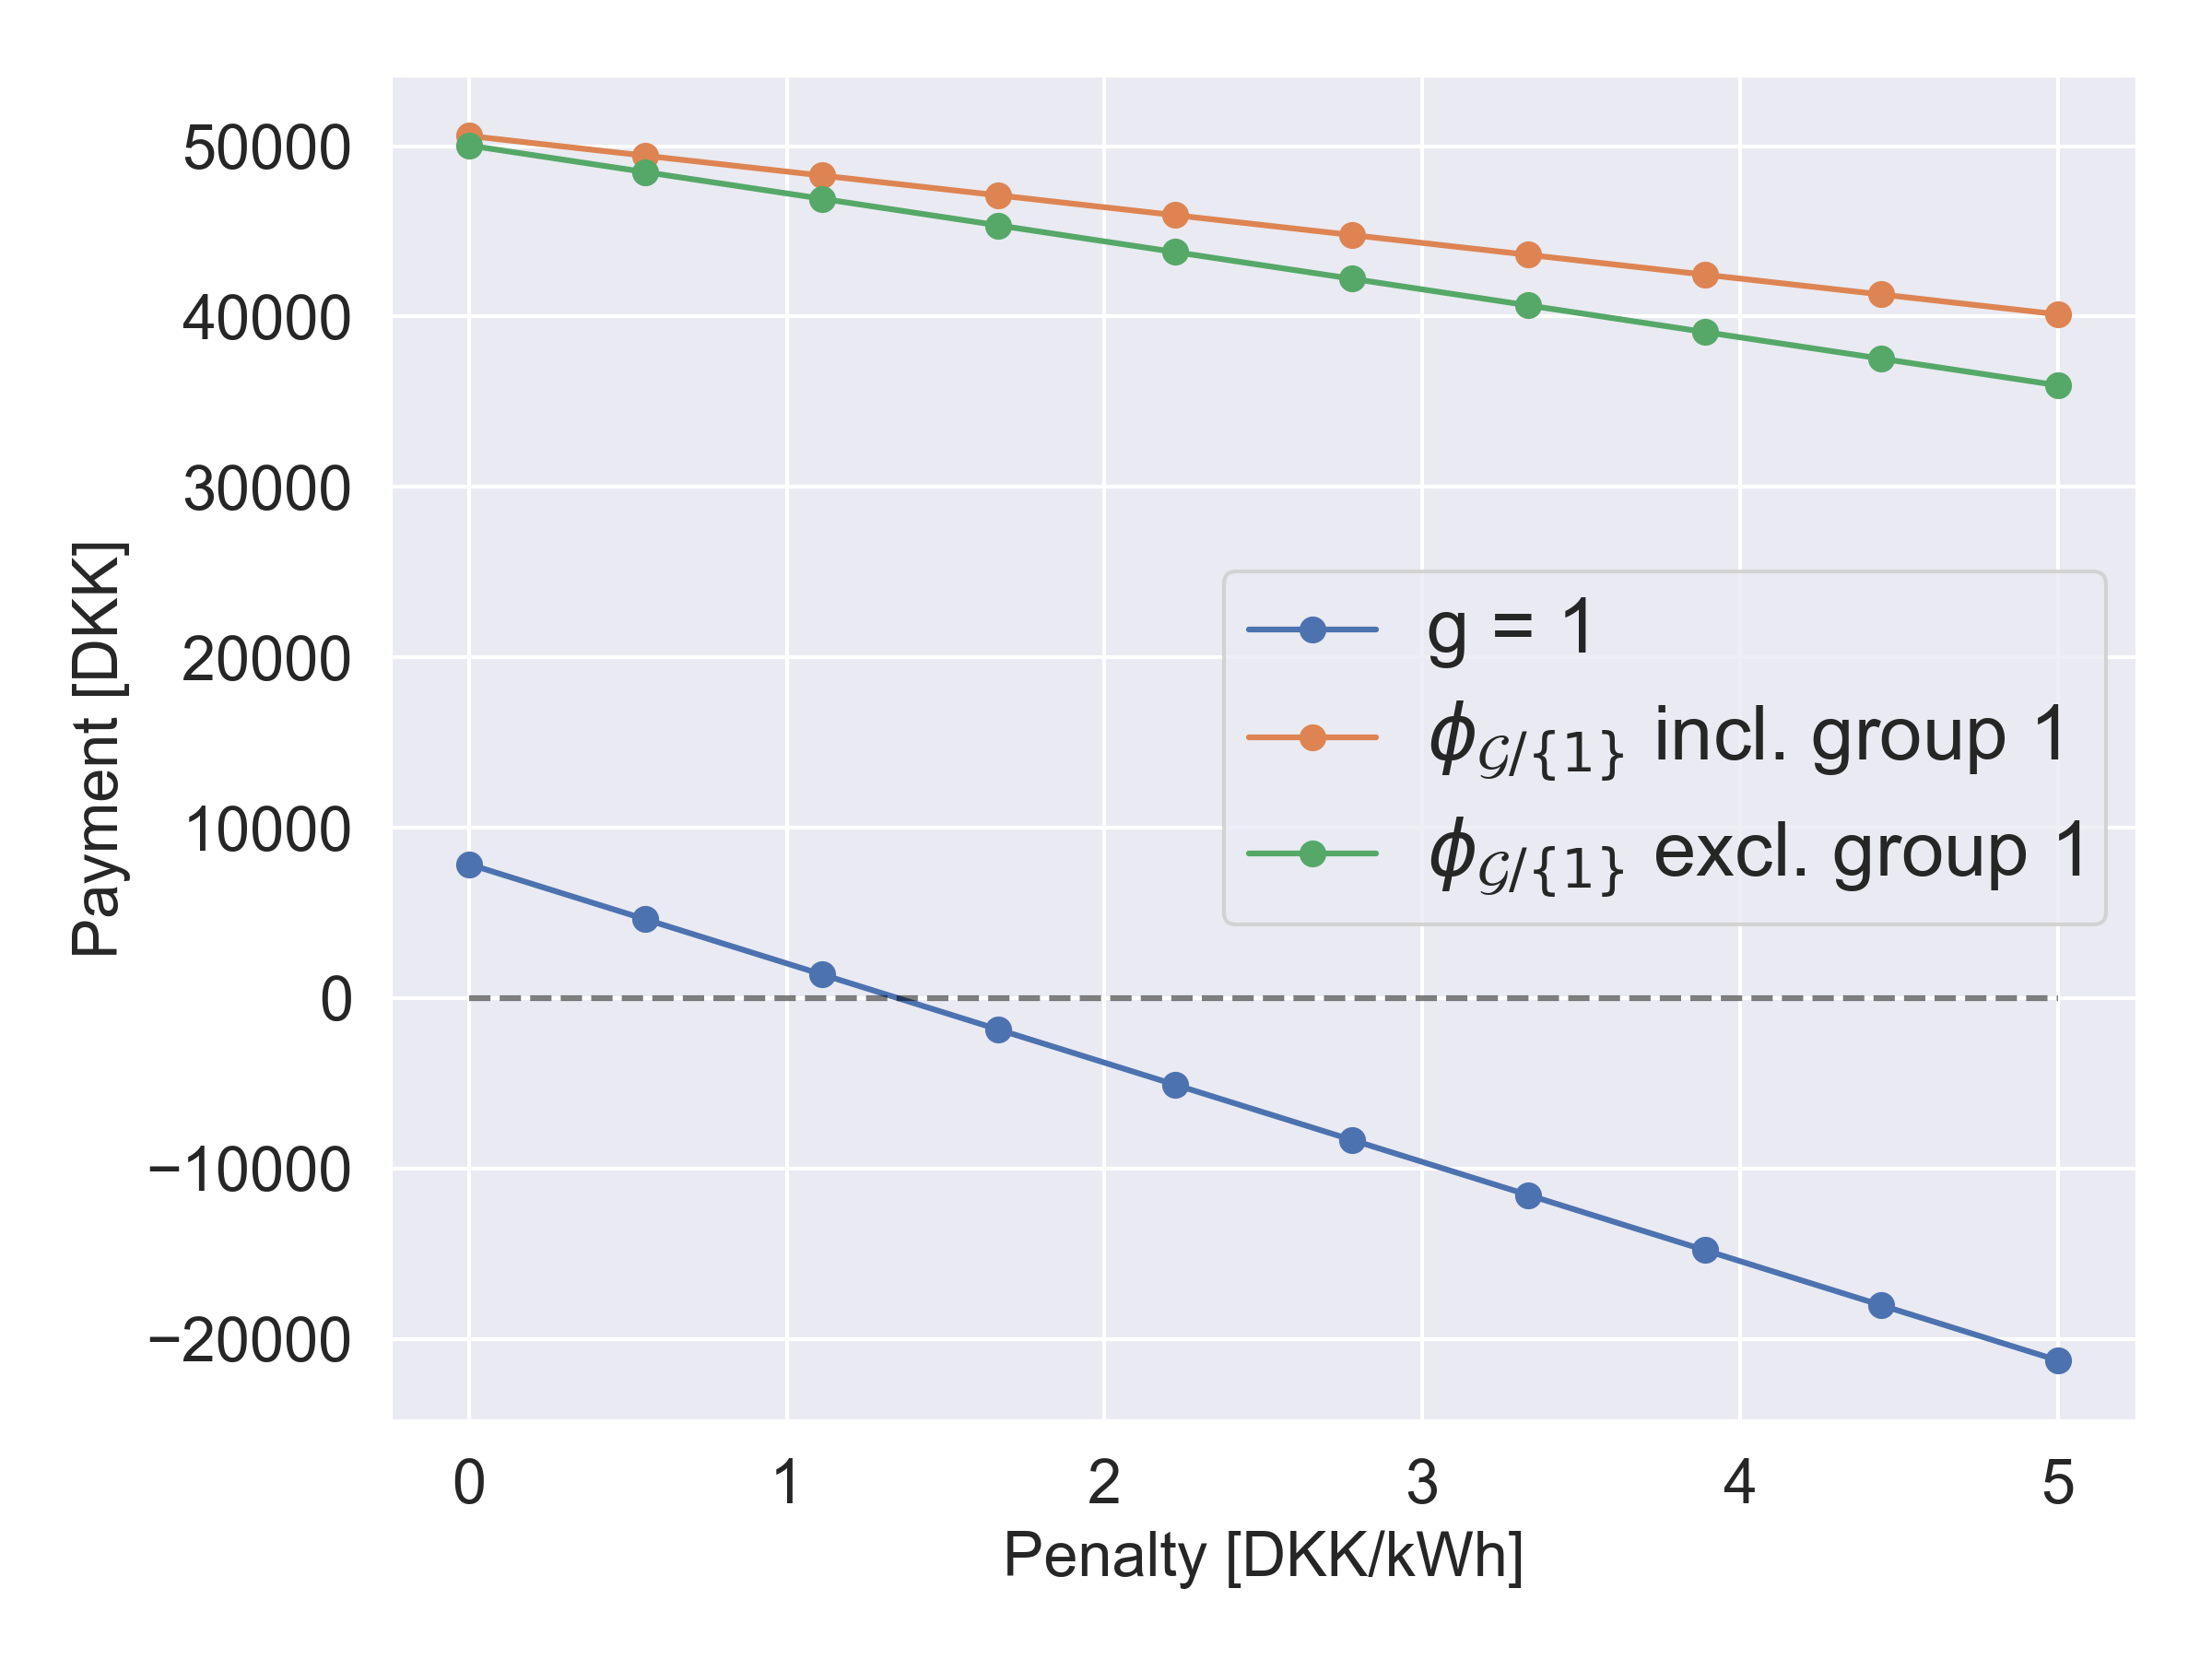
\includegraphics[width=\columnwidth]{figures/shapley_values.png}
    \caption{Simulation of the impact on Shapley values of the penalty price for not delivering promised capacity during up-regulation events. $g_1$ has assets with similar power consumption to $g_{2\hdots 6}$ but never up-regulates. The orange line shows payment to $G / \{1\}$ for the grand coalition, and the green line show payments to them if $g_1$ were not a part of the grand coalition. Likewise, the blue and red lines show payments to $g_1$ when participating in the grand coalition and on its own, respectively.}
    \label{fig:shapley_values}
\end{figure}

\section{Future work}

In this paper, two stylized examples of the same \textit{type} of assets were presented. However, one can also imagine a synergy effect across different types of assets so diversification of the portfolio provides a synergy effect. Hence, dissimilar assets can complement each other. One recent example of this could be Photovoltaic parks providing frequency services in conjunction with batteries or electrolysers increasing profits in synergy with a wind mill and/or batteries.

Moreover, as the number of flexible demands increase, approximate Shapley values must be used. It is interesting to explore how this impacts the fairness and distribution of payments.

\section{Conclusion}

This paper demonstrated the synergy effect of a portfolio of uncertain demand-side assets in terms of numbers in the context of mFRR bidding. Furthermore, flexible demands within an aggregator portfolio, each with such uncertain assets, can be paid fairly using Shapley values. Our simulation showed that flexible demands have individual rationality and thus an incentive to participate in the portfolio as opposed to act on their own. Moreover, a flexible demand that never up-regulates was shown to contribute to the portfolio and get a positive payment when the penalty price for not delivering promised flexibility was low.

\bibliographystyle{IEEEtran}
% \bibliography{tex/bibliography/Bibliography}
\bibliography{bibliography/Bibliography}


\vfill

\end{document}
